%\mbox{}\newpage
\chapter{\hspace{-1mm}\bf 联邦学习仿真系统的设计与实现}
\label{chap5}
\addcontentsline{toe}{chapter}{{{\bf Chapter 5\ \
 Design and Implementation of a Federated Learning Simulation System}}\numberline\,}
\markboth{第\,5\,章\ \
联邦学习仿真软件设计与实现}{北京航空航天大学博士后研究工作报告}

\newcommand{\urlgithub}{\url{https://github.com/wenh06/fl-sim}}
\newcommand{\urlgitee}{\url{https://gitee.com/wenh06/fl-sim}}

%%%%%%%%%%%%%%%%%%%%%%%%%%%%%%%%%%%%%%%%%%%%%%%%%%%%%%%%%%%

\section{仿真系统设计}
\addcontentsline{toe}{section}{{5.1\ \ Design of the Simulation System}\numberline\,}
\label{sec:chap5-design}

% almost finished
% indexed

本文实现的联邦学习仿真系统采用Python语言编写,整体结构借鉴了FedML\footnote{\url{https://github.com/FedML-AI/FedML}}\parencite{he_2020_fedml},\texttt{FedProx}\footnote{\url{https://github.com/litian96/FedProx}}\parencite{sahu2018fedprox}以及pFL-Bench\footnote{\url{https://github.com/alibaba/FederatedScope/tree/master/benchmark/pFL-Bench}}\parencite{chen_2022_pfl_bench}。实现的基本思路是基于配置文件 (或者Python类),将数据集读取、模型参数初始化、节点分配等工作自动化。同时将节点与算法解耦合,节点需要执行的通用操作,例如通讯、获取模型参数等进行统一实现,算法相关的操作通过预留接口的方式完成。这样,利用这一套仿真系统,可以专注于联邦学习优化算法的实现与验证工作。

本文实现的联邦学习仿真系统主要包含以下几个模块
\begin{itemize}
    \item \texttt{data\_processing}: 联邦学习数据集数据处理模块,主要基于已有的一些研究型联邦学习框架LEAF\cite{caldas2018_leaf},应用型联邦学习框架FedML\cite{he_2020_fedml},以及之前的一些联邦学习领域影响力较大的工作\cite{mcmahan2017fed_avg,sahu2018fedprox,reddi2020fed_opt}提出的联邦数据集,包括图像分类的数据集MNIST\cite{Lecun_1998_mnist}, EMNIST\cite{cohen2017emnist}, Federated-EMNIST\cite{caldas2018_leaf,sahu2018fedprox},文本情感分类数据集Sent140\cite{sent140,caldas2018_leaf},文本数据集Shakespeare (用于下一字符预测任务, Next Character Prediction)\cite{mcmahan2017fed_avg,caldas2018_leaf}等。每一个数据集以Python类的形式提供,其中打包了数据集自动下载,数据预处理(例如图像数据增强、归一化以及文本数据的向量化等操作),为节点分配数据,创建模型训练用的数据加载器 (PyTorch DataLoader),计算模型预测结果指标 (例如平均损失 (Mean Loss),准确度 (Accuracy) 等) 等功能,并提供了该数据集常用模型的列表供选择使用。本文随后的章节\S\ref{sec:chap5-datasets}将对已集成的联邦学习数据集进行更具体的介绍。
    \item \texttt{models}: 此模块主要聚合了一些已有的联邦学习文献\cite{mcmahan2017fed_avg,zhang2020fedpd,sahu2018fedprox,Ghosh_2022_cfl,he_2020_fedml}中使用过的试验模型,包括一些卷积神经网络 (Convolutional Neural Network, CNN)\index{卷积神经网络, Convolutional Neural Network, CNN}, 循环神经网络 (Recurrent Neural Network, RNN)\index{循环神经网络, Recurrent Neural Network, RNN},多层感知机 (Multi-Layer Perceptron, MLP)\index{多层感知机, Multi-Layer Perceptron, MLP} 等,为\texttt{data\_processing}模块中的数据集提供备选的试验模型。
    \item \texttt{optimizers}: (子节点上的) 内循环问题求解器。由于大部分试验用模型是神经网络模型,内循环问题的求解大部分基于随机梯度下降算法,包括临近问题的求解,拉格朗日函数的求解。大部分求解器支持方差缩减技术的应用。
    \item \texttt{algorithms}: 这一模块包含了基于本文构建的联邦学习仿真系统复现的部分典型的联邦学习算法,可以用作基准对比算法。本文已复现的联邦学习算法详细信息见表~\ref{tab:algorithms}.
\end{itemize}

\begin{table}[htbp]
\centering
\begin{threeparttable}[b]
\begin{tabular}{|c|c|c|}
\hlineB{3.5}
算法 & 发表杂志/会议 & 官方代码库 \\
\hline \hline
\href{https://github.com/wenh06/fl-sim/tree/master/fl_sim/algorithms/fedprox}{\texttt{FedProx}} & \href{https://proceedings.mlsys.org/paper_files/paper/2020/hash/1f5fe83998a09396ebe6477d9475ba0c-Abstract.html}{MLSys2020}\cite{sahu2018fedprox} & \url{https://github.com/litian96/FedProx} \\
\href{https://github.com/wenh06/fl-sim/tree/master/fl_sim/algorithms/fedopt}{\texttt{FedOpt}}\tnote{$\ast$} & \href{https://arxiv.org/abs/2003.00295}{arXiv:2003.00295}\cite{reddi2020fed_opt} & N/A \\
\href{https://github.com/wenh06/fl-sim/tree/master/fl_sim/algorithms/pfedme}{\texttt{pFedMe}} & \href{https://proceedings.neurips.cc/paper_files/paper/2020/hash/f4f1f13c8289ac1b1ee0ff176b56fc60-Abstract.html}{NeurIPS2020}\cite{t2020pfedme} & \url{https://github.com/CharlieDinh/pFedMe} \\
\href{https://github.com/wenh06/fl-sim/tree/master/fl_sim/algorithms/fedsplit}{\texttt{FedSplit}} & \href{https://proceedings.neurips.cc/paper/2020/hash/4ebd440d99504722d80de606ea8507da-Abstract.html}{NeurIPS2020}\cite{pathak2020fedsplit} & N/A \\
\href{https://github.com/wenh06/fl-sim/tree/master/fl_sim/algorithms/feddr}{\texttt{FedDR}} & \href{https://papers.nips.cc/paper/2021/hash/fe7ee8fc1959cc7214fa21c4840dff0a-Abstract.html}{NeurIPS2021}\cite{tran2021feddr} & \url{https://github.com/unc-optimization/FedDR} \\
\href{https://github.com/wenh06/fl-sim/tree/master/fl_sim/algorithms/fedpd}{\texttt{FedPD}} & \href{https://ieeexplore.ieee.org/document/9556559}{IEEE Trans. Signal Process}\cite{zhang2020fedpd} & \url{https://github.com/564612540/FedPD/} \\
\href{https://github.com/wenh06/fl-sim/tree/master/fl_sim/algorithms/scaffold}{\texttt{SCAFFOLD}} & \href{https://proceedings.mlr.press/v119/karimireddy20a.html}{PMLR}\cite{karimireddy2020scaffold} & N/A \\
\href{https://github.com/wenh06/fl-sim/tree/master/fl_sim/algorithms/proxskip}{\texttt{ProxSkip}} & \href{https://proceedings.mlr.press/v162/mishchenko22b.html}{PMLR}\cite{proxskip} & N/A \\
\href{https://github.com/wenh06/fl-sim/tree/master/fl_sim/algorithms/ditto}{\texttt{Ditto}} & \href{https://proceedings.mlr.press/v139/li21h.html}{PMLR}\cite{li_2021_ditto} & \url{https://github.com/litian96/ditto} \\
\href{https://github.com/wenh06/fl-sim/tree/master/fl_sim/algorithms/ifca}{\texttt{IFCA}} & \href{https://papers.nips.cc/paper_files/paper/2020/hash/e32cc80bf07915058ce90722ee17bb71-Abstract.html}{NeurIPS2020}\cite{Ghosh_2022_cfl} & \url{https://github.com/jichan3751/ifca} \\
\href{https://github.com/wenh06/fl-sim/tree/master/fl_sim/algorithms/pfedmac}{\texttt{pFedMac}} & \href{https://arxiv.org/abs/2107.05330}{arXiv:2107.05330}\cite{li2021pfedmac} & N/A \\
\hlineB{3.5}
\end{tabular}
\begin{tablenotes}
\item[$\ast$] \texttt{FedAvg} (还包括\texttt{FedAdam}、\texttt{FedYogi}等) 是\texttt{FedOpt}的特例。
\end{tablenotes}
\caption{基于本文开发的联邦学习仿真系统复现的典型联邦学习算法}
\label{tab:algorithms}
\end{threeparttable}
\end{table}


我们定义了一个抽象基类 (Abstract Base Class, ABC)\index{抽象基类, Abstract Base Class, ABC} \texttt{Node}作为子节点的类\texttt{Client}以及中心节点\texttt{Server}的公共基类,实现了所有类型的节点都要执行的公有操作:
\begin{itemize}
    \item \texttt{get\_detached\_model\_parameters}:获取当前节点分离形式 (即从PyTorch的计算图 (Computation Graph) \index{计算图, Computation Graph}) 的模型参数。
    \item \texttt{get\_gradients}:获取当前被训练模型 (或者说目标函数) 的梯度,或者梯度的范数。
\end{itemize}
同时,以抽象方法 (Python abstractmethod) 的形式,约定所有类型的节点都必须实现的操作,包括
\begin{itemize}
    \item \texttt{communicate}: 节点间通信的操作。
    \item \texttt{update}: 节点执行迭代,更新节点上各种类型参数 (主要是更新正在训练的模型参数,以及对偶参数等) 的操作。
    \item \texttt{\_post\_init}, \texttt{required\_config\_fields}: 检查初始化是否合法相关的操作。
\end{itemize}

中心节点基类\texttt{Server}以及子节点基类\texttt{Client}分别继承\texttt{Node}基类,实现相应类型节点公有的一些操作。其中,中心节点基类\texttt{Server}实现的主要公有操作有:
\begin{itemize}
    \item \texttt{\_setup\_clients}, \texttt{\_allocate\_devices}: 为子节点分配训练数据,初始化模型参数,分配内存或显存空间等。
    \item \texttt{\_sample\_clients}: 对节点进行随机采样,以供参与当前轮次的模型训练。
    \item \texttt{add\_parameters}, \texttt{avg\_parameters}: 从收集到的子节点模型的信息更新全局模型。
    \item \texttt{train}:模型训练的主循环,即图\ref{fig:broadcast-local-update}~与图\ref{fig:agg-global-update}~所示的完整循环。同时,\texttt{train}还额外实现了数据聚合在一起的中心化训练以及无通信的子节点本地训练两种模式,供试验对比效果。
\end{itemize}
子节点基类\texttt{Client}实现的主要公有操作有:
\begin{itemize}
    \item \texttt{evaluate}:利用子节点本地数据对当前模型进行评测。
    \item \texttt{set\_parameters}: 对子节点的本地模型参数进行赋值。这一操作主要是在子节点收到中心节点的全局模型参数等信息后,对本地模型进行更新。
\end{itemize}
利用本文实现的联邦学习仿真系统具体实现某一个算法的时候,只需要分别继承\texttt{Server}以及\texttt{Client}这两个类,将算法的主要步骤在之前提到的\texttt{communicate}, \texttt{update}等几个主要的待实现的方法中进行实现即可。

本文实现的联邦学习仿真系统相关的代码地址为:
\begin{itemize}
    \item GitHub: \urlgithub
    \item gitee: \urlgitee
\end{itemize}

\section{联邦学习数据集}
\addcontentsline{toe}{section}{{5.2\ \ Datasets for Federated Learning}\numberline\,}
\label{sec:chap5-datasets}

% NOT finished
% NOT indexed

\begin{table}[htbp]
\centering
\begin{threeparttable}[b]
\begin{tabular}{|c|c|c|c|c|}
\hlineB{3.5}
数据集名称 & 规模 & 默认节点数目 & 任务 & 样本类型 \\
\hline \hline
MNIST\tnote{$\ast$} & 60000 & 1000 & 图像分类 & $28\times 28$的单通道灰度图像 \\
EMNIST\tnote{$\ast$} & 749068 & 3400 & 图像分类 & $28\times 28$的单通道灰度图像 \\
CIFAR10/100 & 60000 & 500 & 图像分类 & $32\times 32$的RGB3通道图像 \\
Shakespeare & 18424 & 715 & 下一字符预测 & 文本 \\
Sent140 & 40783 & 715 & 文本情感分类 & 文本 \\
Synthetic($\alpha, \beta$)\tnote{$\ast\ast$} & N/A & N/A & 分类 & 随机生成的高维向量 \\
\hlineB{3.5}
\end{tabular}
\begin{tablenotes}
\item[$\ast$] {\smaller 这两个数据集还有经过筛选\cite{sahu2018fedprox}的规模更小的数据子集,也被本文实现的联邦学习仿真系统所包含。}
\item[$\ast\ast$] {\smaller 参数$\alpha, \beta$是两个独立的均值为$0$的正态分布的标准差,用于模拟节点内以及节点间的数据分布差异。}
\end{tablenotes}
\caption{本文开发的联邦学习仿真系统内置的数据集}
\label{tab:datasets}
\end{threeparttable}
\end{table}


\begin{figure}[H]
\centering
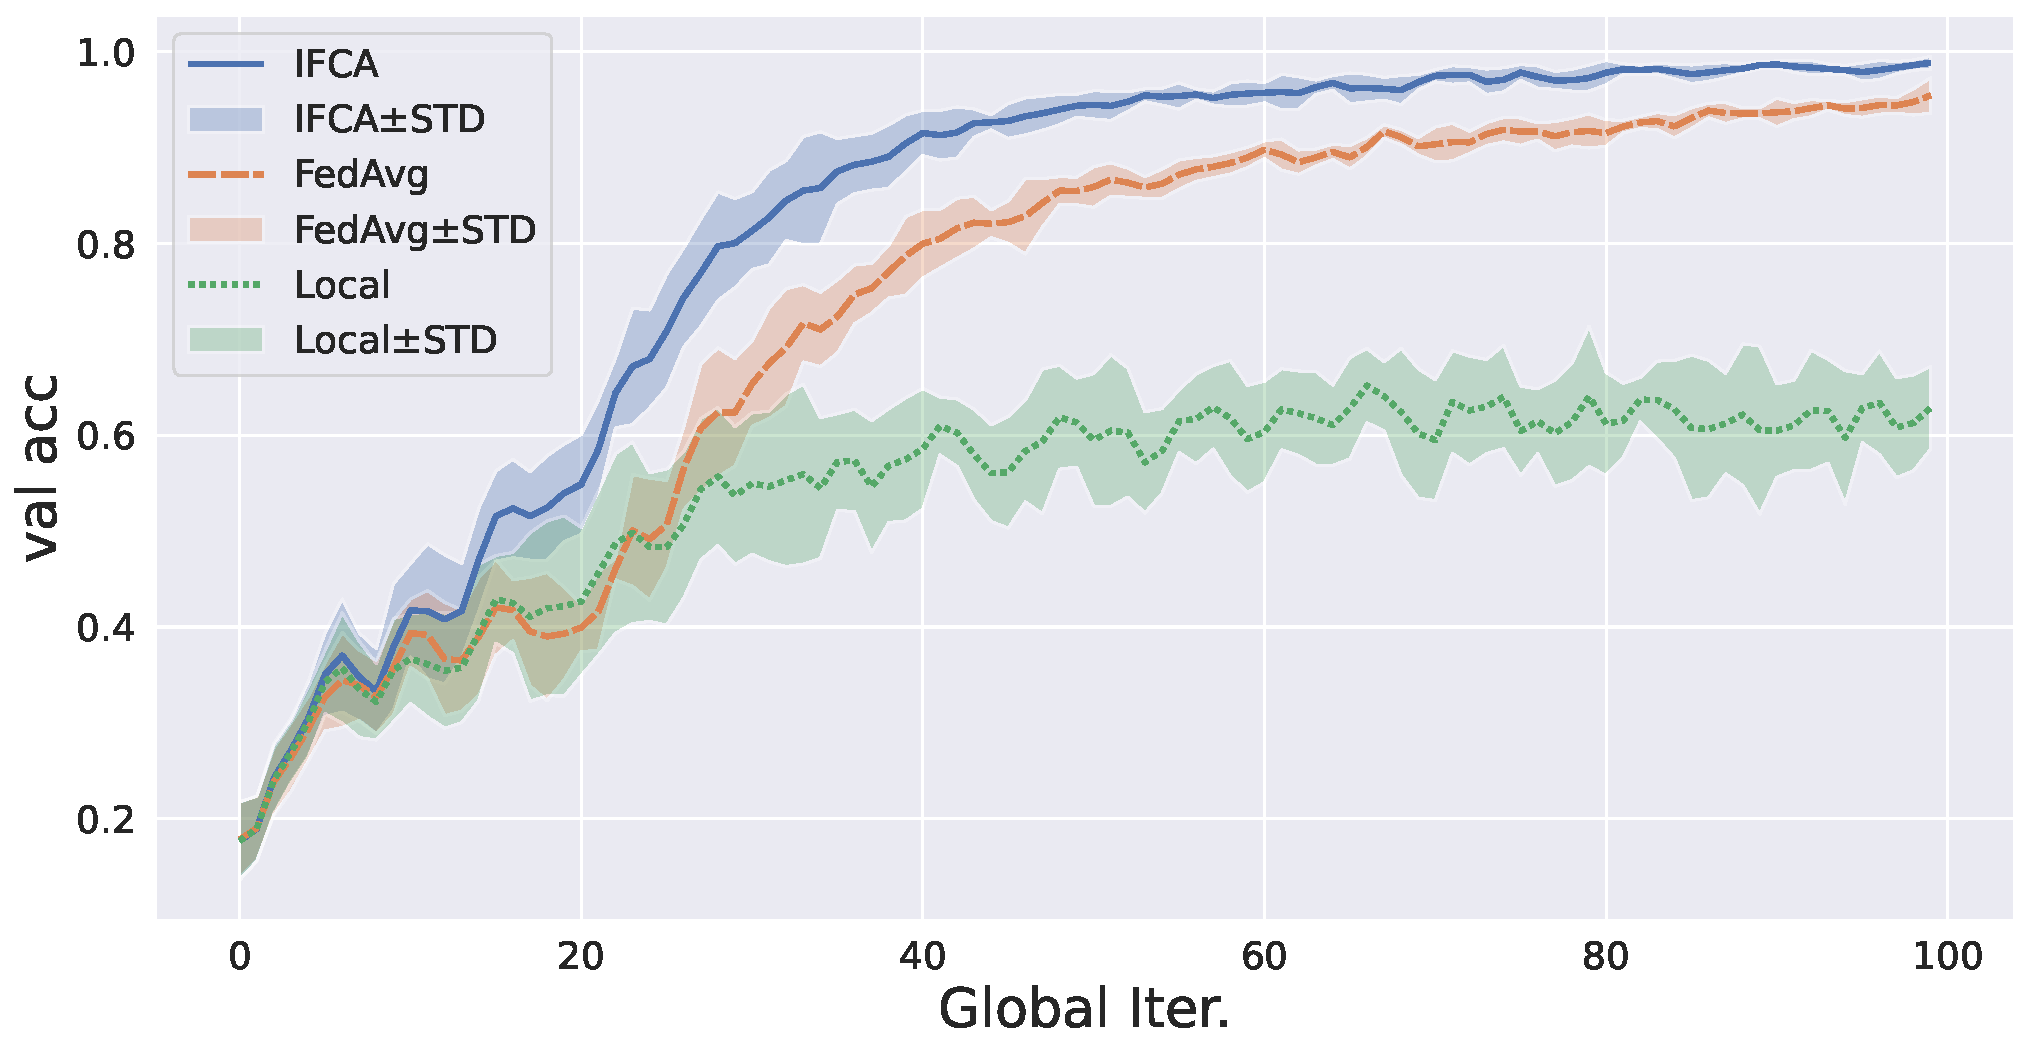
\includegraphics[width=\textwidth]{figures/fedproxfemnist.pdf}
\caption{待写}
\label{fig:fedproxfemnist-experiment}
\end{figure}

待写。。。。

\section{可视化}
\addcontentsline{toe}{section}{{5.3\ \ Visualization}\numberline\,}
\label{sec:chap5-visualization}

% NOT finished
% NOT indexed

\begin{figure}[H]
    \centering
    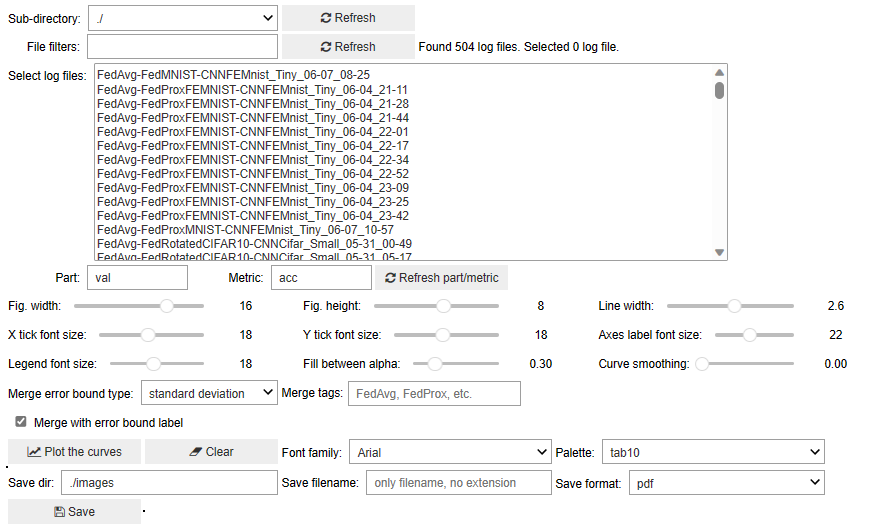
\includegraphics[width=\textwidth]{figures/panel-init.png}
    \caption{待写}
    \label{fig:panel-init}
\end{figure}

\begin{figure}[H]
    \centering
    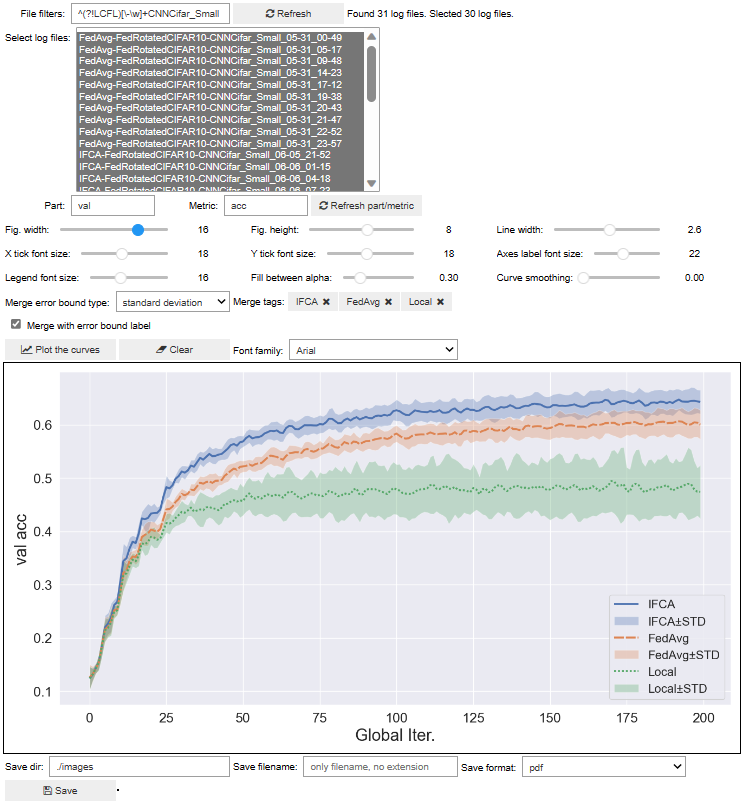
\includegraphics[width=\textwidth]{figures/panel-in-use.png}
    \caption{待写}
    \label{fig:panel-in-use}
\end{figure}

待写。。。。
